% !TEX encoding = UTF-8 Unicode

\documentclass{article}
\usepackage[french]{babel}
\author{Louis DESVERNOIS, Alexis SCHOENN, Philippe DUBOIS}
\title{%
    SAÉ24: Web \\
    \large Groupe 13}
% \date{9 Juin 2022}
\usepackage[left=2.5cm,right=2.5cm,top=2.5cm,bottom=2.5cm]{geometry}
\usepackage{subcaption}
\usepackage{listings}
\usepackage{minted}
\usepackage{graphicx}
\usepackage[T1]{fontenc}
\usepackage[colorlinks=true,linkcolor=black,anchorcolor=black,citecolor=black,filecolor=black,menucolor=black,runcolor=black,urlcolor=black]{hyperref}

%\setcounter{tocdepth}{1} % pour la profondeur de la ToC

\usepackage{fancyhdr}
\pagestyle{fancy}
\fancyhf{}
\renewcommand{\headrulewidth}{0pt}
\rfoot{\thepage}
\lfoot{SAÉ24: Groupe 13}

\renewcommand{\listoflistingscaption}{Table des codes}
\renewcommand{\listingscaption}{Code}

\begin{document}

\maketitle
\tableofcontents
\listoffigures
\listoflistings

\newpage
\section{Introduction}
Nous avons créé un site web dynamique avec le framework Django pour afficher les données récupérées par le script de collecte MQTT.
Notre site doit être capable d'afficher les données avec plusieurs filtres et nous devons être capables de modifier le nom et l'emplacement de chaque capteurs.

\section{Base de données}
\subsection{Mise en place du serveur MySQL}
Nous avons utilisé MySQL Workbench pour créer le serveur ainsi que pour le configurer.
Workbench n'est qu'une interface graphique à MySQL, mais n'est pas nécessaire une fois le serveur configuré.
Pour commencer il faut installer le serveur MySQL sur notre machine Windows en le téléchargeant sur le site officiel de MySQL, le programme est activé automatiquement.
Une fois le serveur installé et activé nous devons nous connecter avec Workbench.
\begin{figure}[H]
    \begin{center}
        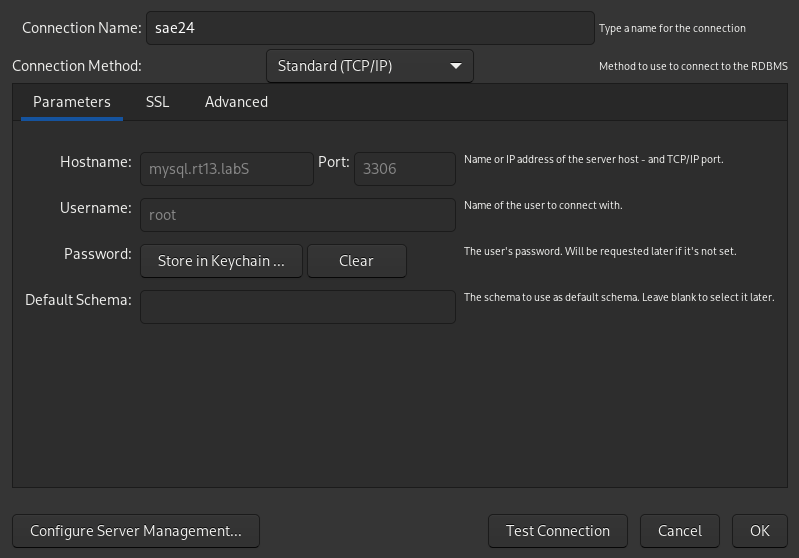
\includegraphics[width=0.7\linewidth]{fig/workbench-conn.png}
    \end{center}
    \caption{Connexion à la BDD avec Workbench}
    \label{workbench:conn}
\end{figure}
Dans la Figure \ref{workbench:conn}, le serveur MySQL est déjà configuré pour accepter les connexions extérieures, pour activer cela, il faut naviguer dans le menu \emph{Server} puis \emph{Users and Privileges} et configurer le paramètre \emph{Limit to Host Matching} pour le bon utilisateur. En Figure \ref{workbench:ip-matching} nous avons configuré l'accès au VLAN server uniquement avec le \emph{wildcard} \verb|%|.
\begin{figure}[H]
    \begin{center}
        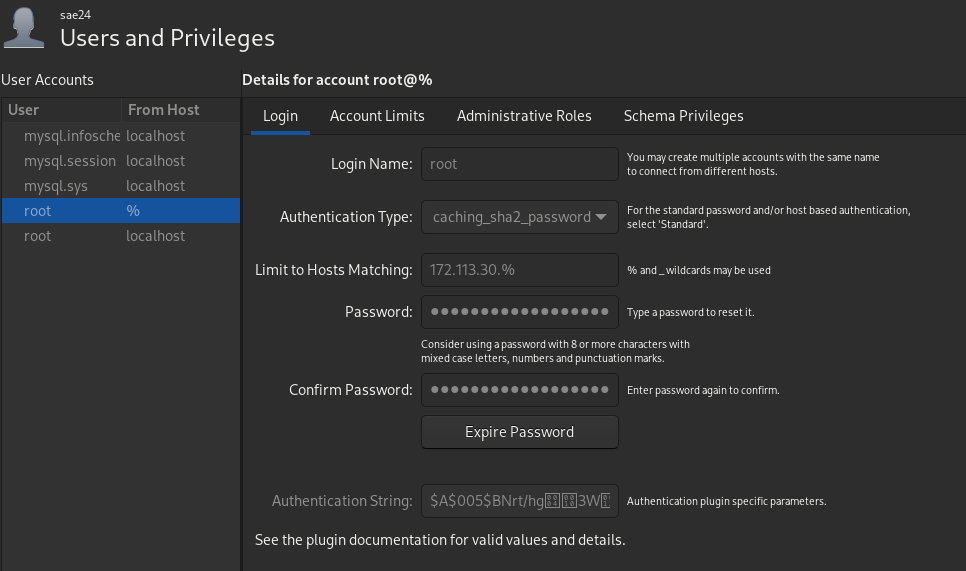
\includegraphics[width=0.7\linewidth]{fig/workbench-allow-ip.png}
    \end{center}
    \caption{Paramétrage de l'accès à distance}
    \label{workbench:ip-matching}
\end{figure}

\subsection{Création de la base de données et des tables}
La base de données ainsi que les tables sont créés dans notre script de collecte MQTT avec des requêtes SQL.
\begin{listing}[H]
    \begin{minted}[breaklines]{sql}
CREATE DATABASE temp;
USE temp;

CREATE TABLE IF NOT EXISTS temp.sensors (
    id INT NOT NULL AUTO_INCREMENT,
    macaddr VARCHAR(12) NOT NULL,
    piece VARCHAR(50) NOT NULL,
    emplacement VARCHAR(50),
    nom VARCHAR(50),
    UNIQUE (macaddr),
    PRIMARY KEY (id));

CREATE TABLE IF NOT EXISTS temp.sensors_data (
    id INT NOT NULL AUTO_INCREMENT,
    sensor_id INT NOT NULL,
    CONSTRAINT sensorFK
        FOREIGN KEY (sensor_id)
        REFERENCES temp.sensors(id),
    datetime DATETIME NOT NULL,
    temp FLOAT NOT NULL,
    PRIMARY KEY (id));
    \end{minted}
    \caption{Création de la base de données et des tables}
    \label{bdd:creation}
\end{listing}

\section{Création projet Django}
\subsection{}

\end{document}